\begin{ledgroupsized}[r]{120mm}
\footnotesize
\pstart
\noindent\textbf{\"{U}berlieferung:}   
\pend
\end{ledgroupsized}
\begin{ledgroupsized}[r]{114mm}
\footnotesize
\pstart
\parindent -6mm
\makebox[6mm][l]{\textit{L}}Konzept: LH XXXVII 5 Bl. 4-5, 8-9. 2 Bog. 4\textsuperscript{o}. Etwas mehr als 7 S. fortlaufend beschrieben; Bl. 9~v\textsuperscript{o} nach fünf Textzeilen leer. Am oberen linken Rand von Bl. 4~r\textsuperscript{o} der Vermerk: \textit{De motu cogitata confusanea (1)}. Am oberen rechten Rand von Bl. 8~r\textsuperscript{o} der Vermerk: \textit{De motu cogitata confusanea (2)}. Auf Bl. 8~r\textsuperscript{o} befindet sich zudem eine gestrichene Zeichnung, die keinen erkennbaren Zusammenhang mit dem Text aufweist und am Ende des St\"{u}cks nachgebildet wird. \"{A}hnliche Zeichnungen sind in N. ?? [[Wallis-Exerpt.]] und N. ?? [[35.13.3,35v]] anzutreffen, an beiden Stellen im Zusammenhang mit \"{U}berlegungen zum Perpetuum mobile. Die Zeichnungen [\textit{Fig. 13}] und [\textit{Fig. 14}] sind durch Papierverlust leicht besch\"{a}digt. Die Bogen, s\"{a}mtlich durch Papiererhaltungsma{\ss}nahmen gesichert, tragen mittig verschiedene Wasserzeichentypen. \\Cc 2, Nr. 945 A
\pend
\end{ledgroupsized}

%\normalsize
\vspace*{5mm}
\begin{ledgroup}
\footnotesize 
\pstart
\noindent\footnotesize{\textbf{Datierungsgr\"{u}nde}: Das vorliegende St\"{u}ck N. ??R/1 befasst sich versuchsweise mit dem Ph\"{a}nomen der Reibung als Ursache von Verz\"{o}gerung bei der Bewegung von K\"{o}rpern in widerstehenden Medien. Die Thematik wird vorwiegend im Zusammenhang mit theoretischen Ans\"{a}tzen zum Sto{\ss} elastischer K\"{o}rper behandelt. Hierbei unterscheidet sich N. ??R/1 von den eigenh\"{a}ndig auf April 1675 datierten St\"{u}cken N. ??R/2 und ??R/3 vornehmlich dadurch, dass noch keine auf die logarithmische Funktion rekurrierende geometrische Beschreibung der durch die Reibung verursachten Verz\"{o}gerung unternommen wird. Diese Beschreibungsmethode wird indessen in allen sp\"{a}teren St\"{u}cken \"{u}ber die Reibung angewendet. Dies legt nahe, N. ??R/1 f\"{u}r fr\"{u}her als N. ??R/2 und ??R/3 zu halten. Die Bl. 4-5 weisen ferner ein Wasserzeichen auf, das auch in N. ??R/2 (LH XXXVII 5, Bl. 12) und ??R/3 (LH XXXVII 5, Bl. 6) anzutreffen ist. Es ist demnach zu vermuten, dass der entsprechende Text nicht viel fr\"{u}her entstanden ist. Die Bl. 8-9 weisen hingegen das gleiche Wasserzeichen wie das sp\"{a}tere St\"{u}ck N. ??R/7 auf. Dies kann als Indiz daf\"{u}r betrachtet werden, dass die Bl. 4-5 einerseits und die Bl. 8-9 andererseits nicht exakt zur gleichen Zeit verfasst wurden. Daher erweist sich editorisch als ratsam, N. ??R/1 entsprechend zu unterteilen. Der enge inhaltliche Zusammenhang von [\textit{Teil 1}] und [\textit{Teil 2}] erhellt jedoch schon daraus, dass Leibniz die Texttr\"{a}ger nummeriert und mit dem gleichen Vermerk \textit{De motu cogitata confusanea} versehen hat. Die zeitliche N\"{a}he der verwendeten Wasserzeichen zu sp\"{a}teren St\"{u}cken \"{u}ber die Reibung ist schlie{\ss}lich Grund f\"{u}r die Annahme, dass das St\"{u}ck N. ??R/1 insgesamt entweder im April 1675 oder in den Monaten zuvor entstanden ist.}
\pend
\end{ledgroup}

\vspace*{8mm}
\newpage
\pstart
\begin{center}
 [4~r\textsuperscript{o}] De Detrimento Motus\protect\index{Sachverzeichnis}{detrimentum motus}, (:~ab attritu\protect\index{Sachverzeichnis}{attritus}, scilicet~:)
 \end{center}
 \pend
 \pstart
\vspace{0,5em}
\begin{center}
 [\textit{Teil 1}] 
\end{center}
\pend
 

\count\Bfootins=1000
\pstart
\noindent
Esto corpus \textit{A} insistens plano in \edtext{\textit{BC}, cui pondere suo innititur. Ponatur impelli recta \textit{DE}}{\lemma{\textit{BC},}\Bfootnote{\textit{(1)}\ impulsum\protect\index{Sachverzeichnis}{impulsus} \textit{(2)}\ linea \textit{(3)}\ cui recta \textit{DE} \textit{(4)}\ cui [...] innititur. \textit{(a)}\ Hoc si \textit{(b)}\ Ponatur [...] \textit{DE}, \textit{L}}}, sentietur aliqua in propellendo \edtext{difficultas. Primum quaestio est, an si}{\lemma{difficultas.}\Bfootnote{\textit{(1)}\ Equidem \textit{(2)}\ Si \textit{(3)}\ Et etsi \textit{(4)}\ Si \textit{(5)}\ Primum [...] si \textit{L}}} planum ponatur esse perfectum atque ita durum, ut planitiei summa aequalitas nullo incumbentis nisu mutari \edtext{possit, difficultas tamen superfutura sit}{\lemma{possit,}\Bfootnote{\textit{(1)}\ difficultatem tamen superare credo \textit{(2)}\ difficultas [...] sit \textit{L}}}, ab ipso illo nisu unionis, quo corpora jungantur. Sed non arbitror, alioqui \edtext{enim in summe politis}{\lemma{enim}\Bfootnote{\textit{(1)}\ summe polita \textit{(2)}\ in summe politis \textit{L}}}, ut glacies maxima onera non 
     \begin{wrapfigure}{l}{0.47\textwidth}                    
     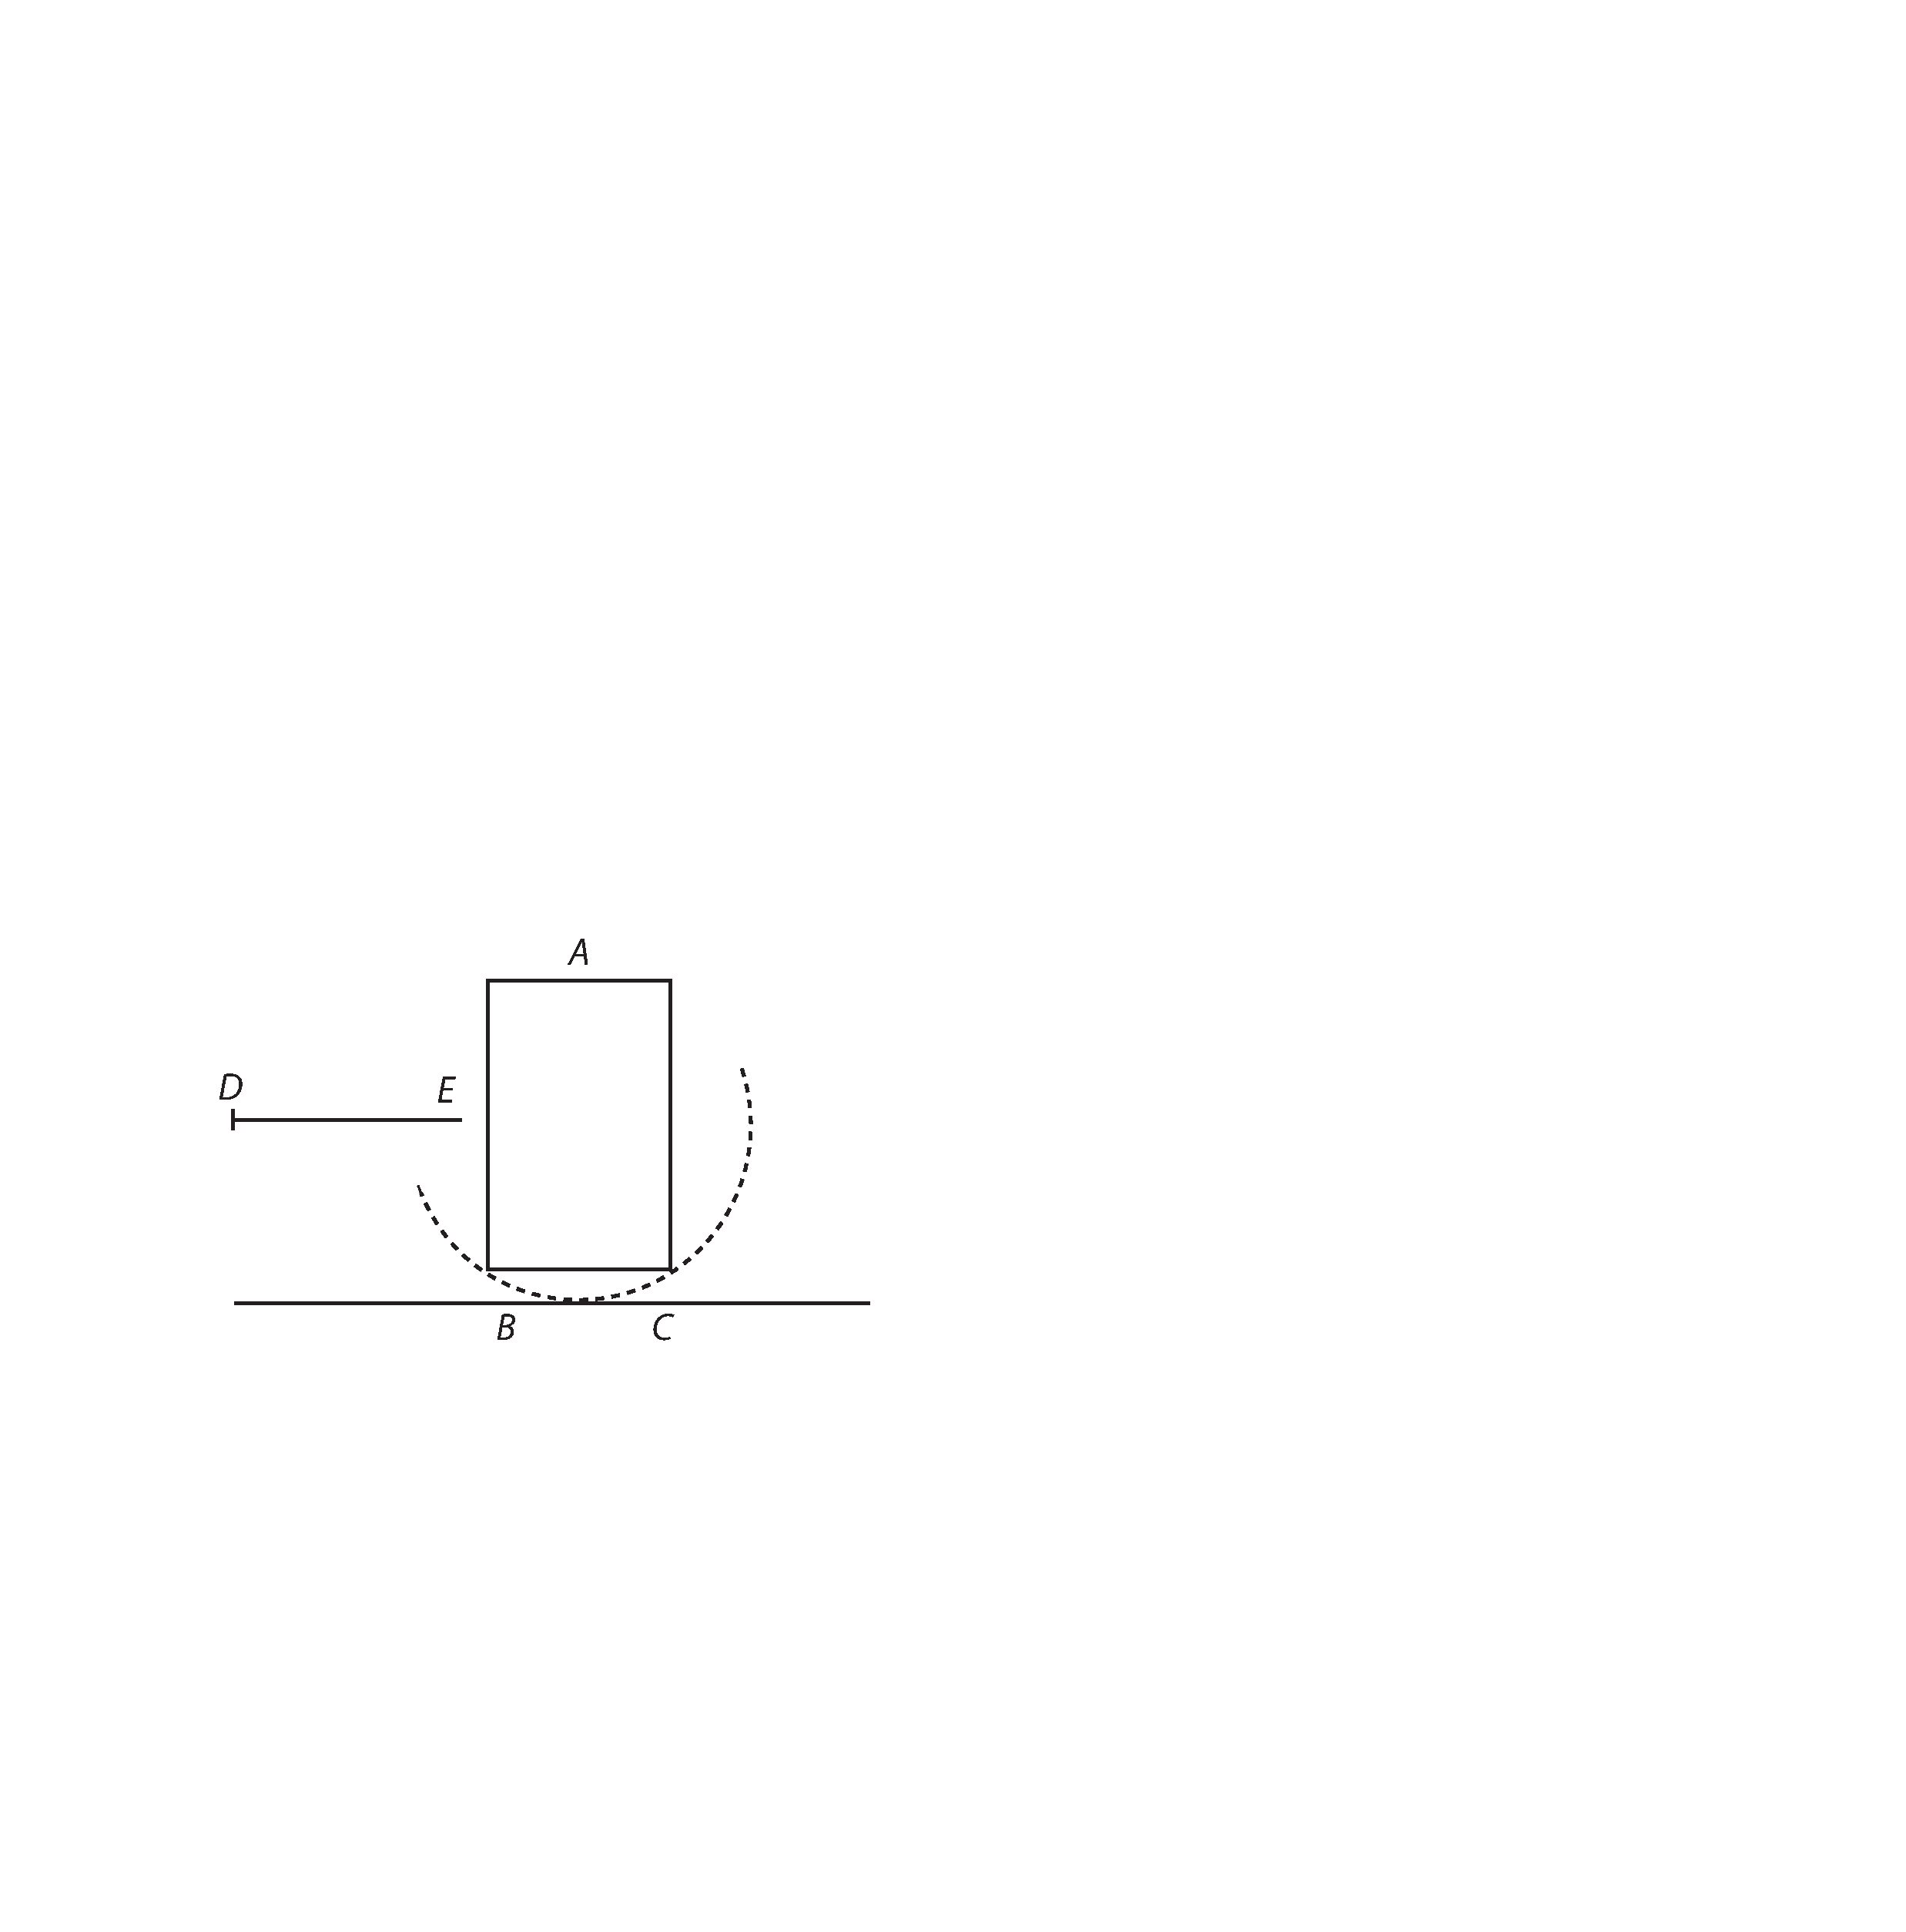
\includegraphics[trim = 48mm 123mm 220mm 205mm, clip, width=0.47\textwidth]{images/lh03705_004r-d1.pdf}
\noindent \centering [\textit{Fig. 1}]
     % \caption{Bildbeschreibung}
     \end{wrapfigure}
\noindent tanta facilitate propellerentur. Et si unionis vis\protect\index{Sachverzeichnis}{vis} a nisu est, tanta foret unio, quantus est nisus, et separare volentibus superandum esset totum corporis pondus\protect\index{Sachverzeichnis}{pondus}, nec facilius esset impellere corpus in glacie aut aqua quam tollere in sublime. Credendum est ergo attritum\protect\index{Sachverzeichnis}{attritus} omnem esse a corporum \edtext{inaequalitate. Aestimanda autem sunt, quantitas contactus, scabrities}{\lemma{inaequalitate.}\Bfootnote{\textit{(1)}\ Pari inaequalitate, sca \textit{(2)}\ Seu scabrities si par est \textit{(3)}\ Seu scabrities \textit{(4)}\ Aestimanda [...] scabrities \textit{L}}}, pondus\protect\index{Sachverzeichnis}{pondus} innitentis, quantitas contactus, nam plurimum interest globum, an cubum propellas; scabrities, nam refert in marmore polito, an in \edtext{tapete globus}{\lemma{tapete}\Bfootnote{\textit{(1)}\ globulus\protect\index{Sachverzeichnis}{globulus} \textit{(2)}\ globus \textit{L}}} \edtext{decurrat}{\lemma{globus}\Bfootnote{\textit{(1)}\ sit \textit{(2)}\ decurrat \textit{L}}}; ac pondus\protect\index{Sachverzeichnis}{pondus} innitentis, nam globus ponderosior caeteris paribus non aeque procurret. Sed re recte \edtext{expensa judico, si corpus, ut globulus decurrat super tapete, nihil conferre ejus pondus}{\lemma{expensa}\Bfootnote{\textit{(1)}\ nihil conferre arbitror pondus\protect\index{Sachverzeichnis}{pondus}, nisi ita \textit{(2)}\ judico [...] ejus pondus \textit{L}}} ad \edtext{attritum\protect\index{Sachverzeichnis}{attritus}, sed}{\lemma{attritum,}\Bfootnote{\textit{(1)}\ consideranda semel \textit{(2)}\ sed \textit{L}}} pondus\protect\index{Sachverzeichnis}{pondus} idem agit etiamsi in vacuo moveretur[;] totam enim vim\protect\index{Sachverzeichnis}{vis} motus statim reducit ad certum moderamen: eaque vis\protect\index{Sachverzeichnis}{vis} obstaculo aliquo recepto, et saepe continuato ut quando in tapete decurrit continue decrescit. Perinde ac \edtext{si}{\lemma{}\Bfootnote{si  \textbar\ in \textit{streicht Hrsg.}\ \textbar\ corpus \textit{L}}} corpus in media aqua \edtext{procurrat. Idem}{\lemma{procurrat.}\Bfootnote{\textit{(1)}\ Sed ita \textit{(2)}\ Idem \textit{L}}} est \edtext{quando globum ponimus}{\lemma{quando}\Bfootnote{\textit{(1)}\ corpus poni \textit{(2)}\ globum ponimus \textit{L}}} decurrere in tabula glutinosa. Sed quando ponimus tabulam esse inaequalem, pondus\protect\index{Sachverzeichnis}{pondus} corporis ad rem pertinere arbitror; majore enim vi\protect\index{Sachverzeichnis}{vis} opus est, ad elevandum corpus, ut exiguum quendam montem superet, quam ad ipsum a glutine avellendum. Ibi enim glutinis tantum vis\protect\index{Sachverzeichnis}{vis} superatur, et corporis in quantum motui in plano resistit pondus\protect\index{Sachverzeichnis}{pondus} ejus. Hic vero ipsum corporis pondus\protect\index{Sachverzeichnis}{pondus}, idem est de alio nisu corporis contra aliud corpus quod contingit, ut chordarum contra rotas. Excutiendum tamen obiter est, antequam \edtext{pergamus, unde}{\lemma{pergamus,}\Bfootnote{\textit{(1)}\ an \textit{(2)}\ unde \textit{L}}} fiat, ut corpus in plano etiam politissimo videatur difficulter propelli posse. Ego non video unde ea resistentia\protect\index{Sachverzeichnis}{resistentia} oriri possit, nisi ab eo qui superest attritu\protect\index{Sachverzeichnis}{attritus}, contra aerem \edtext{planum}{\lemma{}\Bfootnote{planum \textit{erg.} \textit{L}}} et alia corpora per quae decurrit. Pone sagittam\protect\index{Sachverzeichnis}{sagitta} horizontaliter projici, pondus\protect\index{Sachverzeichnis}{pondus} eam tandem ad terram deducit, ita pondus\protect\index{Sachverzeichnis}{pondus} vehae, sive d'un traîneau agens contra inaequalitates glaciei tandem vim\protect\index{Sachverzeichnis}{vis} impressam destruit. Quod longius projicimus pilam\protect\index{Sachverzeichnis}{pila} plumbeam \edtext{quam ligneam,}{\lemma{quam}\Bfootnote{\textit{(1)}\ aeneam, \textit{(2)}\ ligneam, \textit{L}}} ratio esse videtur, quod plumbum\protect\index{Sachverzeichnis}{plumbum} solidius, unde minus in eo materiae extraneae, sive aethereae atque ideo minus attritus\protect\index{Sachverzeichnis}{attritus}, quemadmodum chartam in globulum\protect\index{Sachverzeichnis}{globulus} compressam longius projeceris, quam \edtext{expansam, aut}{\lemma{expansam,}\Bfootnote{\textit{(1)}\ quia \textit{(2)}\ at \textit{(3)}\ aut \textit{L}}} 
\count\Bfootins=1500
ne huic exemplo \edtext{chartae}{\lemma{}\Bfootnote{chartae \textit{erg.} \textit{L}}} latitudinem objicias, longius projicies spongiam compressam, quam dilatatam. Et sane ab ejusmodi detrimento\protect\index{Sachverzeichnis}{detrimentum} oriri pendulorum\protect\index{Sachverzeichnis}{pendulum} et Elateriorum cessationem, aut certe detrimentum\protect\index{Sachverzeichnis}{detrimentum}, videtur manifestum. Satis ergo fortis causa ad rationem reddendam, cur corpora majora difficilius impellantur. Videmus ergo ab Attritu\protect\index{Sachverzeichnis}{attritus} oriri magnorum phaenomenorum% \pend